\section{18.12.23 : Kompleksy podwójne, totalne i inne przymiotniki}
 
\begin{lemma}
  W $K^+(\mathbf{A})$ jeśli $f:X^*\to Y^*$ jest qis, a $I^*$ jest kompleksem injektywnym, to wówczas
  $$Hom_{K^+(\mathbf{A})}(Y^*, I^*)\cong Hom_{K^+(\mathbf{A})}(X^*, U^*)$$
  jest izomorfizmem.
\end{lemma}

\begin{proof}
  Rozważmy trójkąt wyróżniony
  \begin{center}\begin{tikzcd}
    \Delta(f):X^*\arrow[r, "f"] & Y^*\arrow[r] & C(f) \arrow[r] & X^*[1]
  \end{tikzcd}\end{center}
  z niego dostajemy długi ciąg dokładny
  \begin{center}\begin{tikzcd}
    ...\arrow[r] & Hom(X[1], I^*)\arrow[r] & Hom(C(f), I^*)\arrow[r] & Hom(Y^*, I^*)\arrow[r] & Hom(X^*, I^*)\arrow[r] & ... 
  \end{tikzcd}\end{center}
  Udowodnimy, że 
  $$Hom(C(f), I^*)=Hom(C(f)[-1],I^*)=0$$ 
  pokazując, że każdy morfizm z acyklicznego kompleksu $C^*$, na przykład $C(f)$, w $I^*$ jest homotopijny z $0$.

  Ponieważ $f$ jest qis, to 
  $$H^*(C(f))=0$$
  a więc w kolejnym ciągu dokładnym mamy
  \begin{center}\begin{tikzcd}[row sep=tiny]
    ...\arrow[r] & H^i(X^*)\arrow[r] & H^i(Y^*)\arrow[r] & H^i(C(f))\arrow[r] & H^{i+1}(X^*)\arrow[r] & ... \\ 
                & & & \arrow[u, phantom, sloped, "="] 0
  \end{tikzcd}\end{center}

  Niech $g:C^*\to I^*$ i niech $C^*$ będzie acykliczny. Zbudujemy $h:C^*\to I^*[-1]$ takie, że $g^i=dh^i+h^{i+1}d$ indukcyjnie. Dla $i\ll 0$ mamy $h^i=0$:
  \begin{center}\begin{tikzcd}[column sep=large, row sep=large]
    ...\arrow[r] & C^{-1} \arrow[r]\arrow[d, "g^{-1}" left] & C^0 \arrow[r]\arrow[d, "g^0" left]\arrow[dl, "h^0" above left] & C^1 \arrow[r]\arrow[d, "g^1" left]\arrow[dl, "h^1" above left] & ...\\ 
    ...\arrow[r] & 0\arrow[r] & I^0\arrow[r] & I^1\arrow[r] & ...
  \end{tikzcd}\end{center}

  \begin{center}\begin{tikzcd}[column sep=large, row sep=large]
    \arrow[r] & C^{i-1}\arrow[r, "d^{i-1}"]\arrow[d, "g^{i-1}" left] & C^i\arrow[r, "d^i"]\arrow[d, "g^i" left]\arrow[dl, "h^i" above left] & C^{i+1}\arrow[dl, "h^{i+1}" above left] \arrow[r]\arrow[d] & {\color{white}...}\\ 
    \arrow[r] & I^{i-1}\arrow[r, "d" below] & I^i\arrow[r] & I^{i+1}\arrow[r] & {\color{white}...}
  \end{tikzcd}\end{center}
  Załóżmy, że mamy $h^s$ dla $s\leq i$ takie, że $g^{i-1}=dh^{i-1}+h^id$. Chcemy zbudować $h^{i+1}$.
  Pytamy, czy możemy wziąć
  $$h^{i+1}d=g^i-dh^i,$$
  to znaczy, czy tak zdefiniowane $h^{i+1}$ sprawia, że diagram po lewej komutuje, czyli $h^{i+1}dd=0$:
  \begin{align*}
    h^{i+1}dd&=(g^i-dh^i)d=g^id-dh^id=dg^{i-1}-d(g^{i-1}-\underbrace{dh^{i+1}}_{=0})=dg^{i-1}-dg^{i-1}-0=0
  \end{align*}
  Ponieważ
  $$dh^id^{i-1}=g^id^{i-1},$$
  to $(g^i-dh^i)d^{i-1}=0$ i z uniwersalności $\coker$ dostajemy diagram
  \begin{center}\begin{tikzcd}[column sep=large, row sep=large]
    0\arrow[r] & \coker d^{i-1}_c \arrow[r] \arrow[d, "g^i-dh^i" left] & C^{i+1}\arrow[dl, "h^{i+1}", blue] \\ 
               & I^i
  \end{tikzcd}\end{center}
  gdzie niebieska strzałka istnieje, bo $I^i$ jest injektywne. Przemienność tego diagramu mówi, że $g^i-dh^i=h^{i+1}d$, a więc $g^i=dh^i+h^{i+1}d$ tak jak chcieliśmy.
\end{proof}

\begin{conclusion}\label{wniosek 12.2}
  Niech $A^*$ będzie kompelskem, a $I^*\in Kom^+(\mathbf{A})$ będzie injektywny. Wtedy 
  $$Hom_{K^+(\mathbf{A})}(A^*, I^*)=Hom_{D^+(\mathbf{A})}(A^*, I^*)$$
  co wynika z lematu.
\end{conclusion}

\begin{proof}Patrz dowód \ref{wniosek 11.10}
\end{proof}

\subsection{Kompleks podwójny, rezolwenta Cartana-Eilenberga}

\begin{theorem}
  Jeśli w kategorii abelowej $\mathbf{A}$ jest dostatecznie dużo obiektów injektywnych, to funktor włożenia
  $$K^+(\mathbf{I})\to D^+(\mathbf{A})$$
  jest równoważnością kategorii.
\end{theorem}

Zanim przejdziemy do dowodu tego twierdzenia, wprowadzimy kilka przydatnych definicji:

  \begin{definition}[kompleks podwójny, kompleks totalny]
    \buff{Kompleks podwójny} to przemienny diagram $I^{*,*}$ z różniczkami $d_I(\to)$ i $d_{II}(\uparrow)$.

    \buff{Kompleks totalny} kompleksu podwójnego $I^{*,*}$ to 
    $$Tot(I^{*,*})^n=\bigoplus_{i+j=n}I^{i,j}$$
    z różniczką $D=d_I+(-1)^id_{II}$. 
  \end{definition}

  \begin{definition}[rezolwenta Cartana-Eilenberga]\label{rezolwenta C-E}
    Niech $A^*$ będzie kompleksem. Rozważmy kompleks podwójny $I^{*,*}=(I^{i,j})_{i,j\geq 0}$ wyposażony w morfizm $A^*\to I^{*,0}$

    \begin{center}\tikz[overlay]{
      \filldraw[fill=yellow!30, draw=yellow!30, thick, rounded corners](1.6, 2.5) rectangle (2.5, -2.8);
    }
    \begin{tikzcd}
      ... & ... & ... \\ 
      I^{0,2} \arrow[r]\arrow[u] & I^{1,2} \arrow[r]\arrow[u] & I^{2,2}\arrow[r]\arrow[u] & ... \\ 
      I^{0,1}\arrow[r] \arrow[u] & I^{1,1}\arrow[r]\arrow[u] & I^{2, 1} \arrow[r]\arrow[u] & ... \\ 
      I^{0,0}\arrow[r] \arrow[u] & I^{1, 0}\arrow[r]\arrow[u] & I^{2, 0}\arrow[r]\arrow[u] & ... \\ 
      A^0\arrow[u]\arrow[r] & A^1\arrow[r]\arrow[u] & A^2\arrow[r]\arrow[u] & ...
    \end{tikzcd}\end{center}

    Taki kompleks $I^{*,*}$ nazywamy \buff{rezolwentą Cartana-Eilenberga}, jeśli
    \begin{enumerate}
      \item ciągi $\color{orange}A^i\to I^{i,0}\to I^{i, 1}\to I^{i,2} \to ...$ tworzą rezolwenty injektywne $A^i$ "indukujące" rezolwenty injektywne brzegów $B^i$, cykli $Z^i$ i kohomologii $H^i$ kompleksu $A^*$ oraz
      \item różniczki w $I^{*,*}$ oznaczane
    \begin{center}\begin{tikzcd}
      I^{i,j+1} \\ 
      I^{i,j}\arrow[u, "d_{II}^{i,j}"]\arrow[r, "d_I^{i,j}" below] & I^{i+1, j}
    \end{tikzcd}\end{center}
    dają ciągi 
    \begin{center}\begin{tikzcd}
      0\arrow[r] & \ker d^{i,j}_I \arrow[r] & I^{i,j} \arrow[r] & \img d^{i,j}_I\arrow[r] & 0 \\ 
      0\arrow[r] & \img d_I^{i,j}\arrow[r] & \ker d_I^{i+1,j}\arrow[r] & H^{i+1, j}_I\arrow[r] & 0
    \end{tikzcd}\end{center}
    które rozszczepiają się.
\end{enumerate}
  \end{definition}

  Udowodnimy teraz fakt pomocniczy (a raczej lemat), który uprości dowód twierdzenia do znalezienia odpowiedniej rezolwenty Cartana-Eilenberga.

  \begin{fact}\label{qis dla C-E}
  Dla rezolwenty Cartana-Eilenberga morfizm $A^*\to Tot(I^{*,*})$ indukowany przez 
  $$A^*\to I^{*,0}$$ 
  jest qis. 
\end{fact}

Dowodzi się to polowaniem po diagramie, które jest prawdziwe nawet dla sformułowania tego faktu ze słabszymi założeniami:
\begin{lemma}
  Niech $(K^{i,j})_{i,j\geq 0}$ będzie kompleksem podwójnym. $A^*\to K^{*,0}$ to morfizm kompleksów, który uzupełnia kolumny tak, że stają się one dokładne. Wtedy indukowane odwzorowanie $A^*\to Tot(K^{*,*})$ jest qis.
\end{lemma}

\begin{proof}
  {\large\color{red}ZDJĘCIE}

  Zaczynamy od wybrania cyklu $Tot^n$, zaznaczonego na niebiesko. Chcemy pokazać, że istnieje coś w $Z^n(A^*)$ które przechodzi w tenże cykl:
  \begin{center}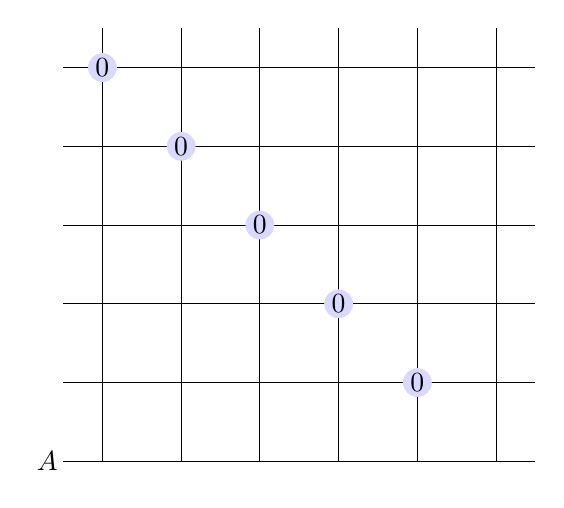
\begin{tikzpicture}
    \foreach \i in {0,...,5}
      { 
        \draw (-0.5,\i)--(5.5, \i);
        \draw (\i, 0)--(\i, 5.5);
      }

      \node at (-0.7, 0) {$A$};

      \foreach \i in {1,...,5}
      {
        \filldraw[blue!15] (5- \i, \i) circle (5pt);
        \node at (5-\i, \i) {$0$};
      }
  \end{tikzpicture}\end{center}
\end{proof}




\begin{proof}
  Wniosek \ref{wniosek 12.2} mówi nam, że funktor wyżej jest wierny i pełny. Pozostaje sprawdzić, że jest w zasadzie surjektywny. To znaczy, że $(\forall\;A^*\in Kom^+(\mathbf{A}))(\exists\;I^*\in Kom^+(\mathbf{A}))$ oraz qis $A^*\to I^*$. Wtedy będziemy mieli izomorfizm w $D^+(\mathbf{A})$.

  Dowód polegać będzie na skonstruowaniu rezolwenty Cartana-Eilenberga.
  \begin{enumerate}
    %\setcounter{enumii}{-1} 
    \item $A\in\ob(\mathbf{A})$ i tworzymy rezolwentę injektywną, bo wiemy, że każdy obiekt wkłada się w jakiś obiekt injektywny.
      \begin{center}\begin{tikzcd}
        0\arrow[r, "i"] & I^0\arrow[rr, "d^0"]\arrow[dr] & & I^1\arrow[rr, "d^1"]\arrow[dr] & & I^2\\ 
                        & & \coker i\arrow[ur] & & \coker d^0\arrow[ur] \\ 
                        & 0\arrow[ur] & & 0\arrow[ur]
      \end{tikzcd}\end{center}
    \item Indukcyjne polowanie po diagramie:
      \begin{center}\begin{tikzcd}
        & 0\arrow[d] & \color{red}0\arrow[d, red] & 0\arrow[d]\\
        0\arrow[r] & B^i\arrow[r]\arrow[d, "\epsilon_B" left] & Z^i\arrow[r]\arrow[dr, red, "j_0"]\arrow[dl, "i_0" above left, dashed, red]\arrow[d, red, "(i_0;j_0)" red] & H^i\arrow[r]\arrow[d, "\epsilon_H"] & 0\\ 
        \color{blue}0\arrow[r, blue] & I^0 \arrow[r, blue] \arrow[d]& \color{blue}I^0\oplus J^0 \arrow[r, blue] & J^0 \arrow[r, blue]\arrow[d] & \color{blue}0\\ 
                   & I^1 & & J^1 
      \end{tikzcd}\end{center}
      Z tego diagramu możemy dostać diagram
      \begin{center}\begin{tikzcd}
        & 0 \arrow[d] & & 0\arrow[d]\\ 
        0\arrow[r] & \coker \epsilon_B\arrow[d] \arrow[r] & \coker (i_0;j_0) \arrow[r] & \coker\epsilon_H \arrow[r]\arrow[d] & 0\\ 
                   & I^1\arrow[d] & indukcja & J^1\arrow[d]\\ 
                   & ... & & ...
      \end{tikzcd}\end{center}
      Dostajemy na koniec diagram 
      \begin{center}\begin{tikzcd}
        & 0\arrow[d] & 0\arrow[d] & 0\arrow[d]\\ 
        0\arrow[r] & B^i\arrow[r]\arrow[d] & Z^i\arrow[r]\arrow[d] & H^i\arrow[r]\arrow[d] & 0\\ 
        0\arrow[r] & I^0\arrow[r]\arrow[d] & I^0\oplus J^0\arrow[r]\arrow[d] & J^0\arrow[r]\arrow[d] & 0\\ 
        0\arrow[r] & I^1\arrow[r]\arrow[d] & I^1\oplus J^1\arrow[r]\arrow[d] & J^1\arrow[r]\arrow[d] & 0\\ 
                   & ... & ... & ...
      \end{tikzcd}\end{center}
    Ciąg 
      $$0\to\img d_I^{i,j}\to \ker d_I^{i,j}\to H_I^{i+1,j}\to 0$$ 
      odpowiada ciągowi 
      $$0\to B^i\to Z^i\to H^i\to 0$$
      natomiast 
      $$0\to \ker d_I^{i,j}\to I^{i,j}\to \img d_I^{i,j}\to 0$$
      odpowiada
      $$0\to Z^i\to A^i\to B^{i+1}\to 0$$
    \item Podobnie jak w poprzednim podpunkcie budujemy rezolwenty $A^*$:
      \begin{center}\begin{tikzcd}
        0\arrow[r] & Z^i\arrow[r]\arrow[d] & A^i\arrow[r]\arrow[d] & B^{i+1}\arrow[r]\arrow[d] & 0\\ 
        0\arrow[r] & I^0\arrow[r]\arrow[d] & I^0\oplus J^0\arrow[r]\arrow[d] & J^0\arrow[r]\arrow[d] & 0\\ 
        0\arrow[r] & I^1\arrow[r]\arrow[d] & I^1\oplus J^1\arrow[r]\arrow[d] & J^1\arrow[r]\arrow[d] & 0\\ 
                                         & ... & ... & ...
      \end{tikzcd}\end{center}
    \item {\large\color{red}ZDJĘCIE}, gdzie to co pod $A$ można na niebiesko, bo to wychodzi z poprzednich podpunktów - tworzy się rezolwenta Cartana-Eilebnerga. plus widzimy te diagramki maluczkie (też na zdjęciu)
  \end{enumerate}
\end{proof}

\subsection{Funktor pochodny}

\begin{definition}[funktor pochodny]
  Niech $F:\mathbf{A}\to\mathbf{B}$ będzie lewo-dokładnym funktorem addytywnym między abelowymi kategoriami. Załóżmy, że w $\mathbf{A}$ jest dostatecznie dużo obiektów injektywnych. \buff{Prawy funktor pochodny}
  $$RF:D^+(\mathbf{A})\to D^+(\mathbf{B})$$
  jest złożeniem diagramów
  \begin{center}\begin{tikzcd}
    K^+(\mathbf{I}_A)\arrow[dr, yshift=-1mm]\arrow[r, hookrightarrow]\arrow[rr, bend left=20, red] & K^+(\mathbf{A}) \arrow[r, "K(F)"]\arrow[d] & K^+(\mathbf{B})\arrow[d]\arrow[d, bend left=20, red]\\
                                                                                                   & D^+(\mathbf{A})\arrow[ul, yshift=1mm]\arrow[ul, bend left=20, red]\arrow[r, red, "RF" below, dashed] & B^+(\mathbf{B})
  \end{tikzcd}\end{center}
\end{definition}
%$RF$ dla $A^*\in\ob D^+(\mathbf{A})$ znajduje qis $A^*\to I^*$ i bierze kompleks $F(I^*$)

\begin{fact}\label{RF dokladny}
  Funktor $RF$ jest dokładny, tzn. przeprowadza trójkąty wyróżnione w $D^+(\mathbf{A})$ na trójkąty wyróżnione w $D^+(\mathbf{B})$.
\end{fact}
\begin{proof}
  Dowód za tydzień.
\end{proof}

\begin{definition}[wyższe funktory pochodne]
  Dla obiektu $A\in\ob\mathbf{A}$ ciąg obiektów
  \begin{align*}
    R^iF(A)&=H^i(RF(A[0]))=\\ 
           &=H^i(F(I^0)\to F(I^1)\to ...)
  \end{align*}
  gdzie $0\to A\to I^0\to I^1$ jest injektywną rezolwentą $A$, nazywamy \buff{wyższym funktorem dokładnym} (lewo-dokładnego) funktora $F$.
\end{definition}

\begin{uwaga}
  $$R^0F(A)=F(A)$$
\end{uwaga}

\begin{proof}
  \begin{center}\begin{tikzcd}
    0\arrow[r] & A\arrow[r] & I^0\arrow[r] & I^1\arrow[r] & ...\\ 
    0\arrow[r] & FA\arrow[r] & FI^0\arrow[r] & FI^1\arrow[r] & ...
  \end{tikzcd}\end{center}
  ponieważ ciąg dokładny przechodzi na ciąg dokładny, to mamy $FA=\ker (FI^0\to FI^1)=R^0F(A)$.
\end{proof}

\begin{fact}
  Jeśli
  \begin{center}\begin{tikzcd}
    0\arrow[r] & A\arrow[r] & B\arrow[r] & C\arrow[r] & 0 
  \end{tikzcd}\end{center}
  jest dokładny w $\mathbf{A}$, to wtedy
  \begin{center}\begin{tikzcd}[row sep=small]
    0\arrow[r] & FA\arrow[r] & FB\arrow[r] & FC\arrow[r]\arrow[d, phantom, ""{coordinate, name=Z}] & R^1FA\arrow[rounded corners, dlll,
    to path={ -- ([xshift=2ex]\tikztostart.east)
      |- ([xshift=2ex, yshift=-3ex]\tikztostart.east)
-| ([xshift=-2ex]\tikztotarget.west)
-- (\tikztotarget)}]
    \\ 
               & R^1FB\arrow[r] & R^1FC\arrow[r] & R^2FA\arrow[r] &...
  \end{tikzcd}\end{center}
  również jest dokładny
\end{fact}

\begin{proof}
  Dla ciągu dokładnego $0\to A\to B\to C\to 0$ mamy trójkąt wyróżniony
  $$\Delta:\;A\to B\to C\to A[1]$$
  a ponieważ $RF$ jest dokładny (\ref{RF dokladny}), to mamy też trójkąt wyróżniony
  $$RF(A)\to RF(B)\to RF(C)\to RF(A)[1]$$
  i długi ciąg $H^*$ związany z przeniesonym $\Delta$, który daje nam już bezpośrednio tezę.
\end{proof}
